
\newcommand{\simforce}[1]{\bm{F}_{\kern -0.02in #1}}

%%%%%%%%%%%%%%%%%%%%%%%%%%%%%%%%%%%%%%%%%%%%%%%%%%%%%%%%%%
%%%%%%%%%%%%%%%%%%%%%%%%%%%%%%%%%%%%%%%%%%%%%%%%%%%%%%%%%%
\chapter[RepulsionPak: Deformation-Driven Element Packing \newline with Repulsion Forces]
{RepulsionPak: Deformation-Driven Element Packing with Repulsion Forces}
\label{chapter_repulsionpak}
%%%%%%%%%%%%%%%%%%%%%%%%%%%%%%%%%%%%%%%%%%%%%%%%%%%%%%%%%%
%%%%%%%%%%%%%%%%%%%%%%%%%%%%%%%%%%%%%%%%%%%%%%%%%%%%%%%%%%

\begin{figure*}[h!]
  \centering
  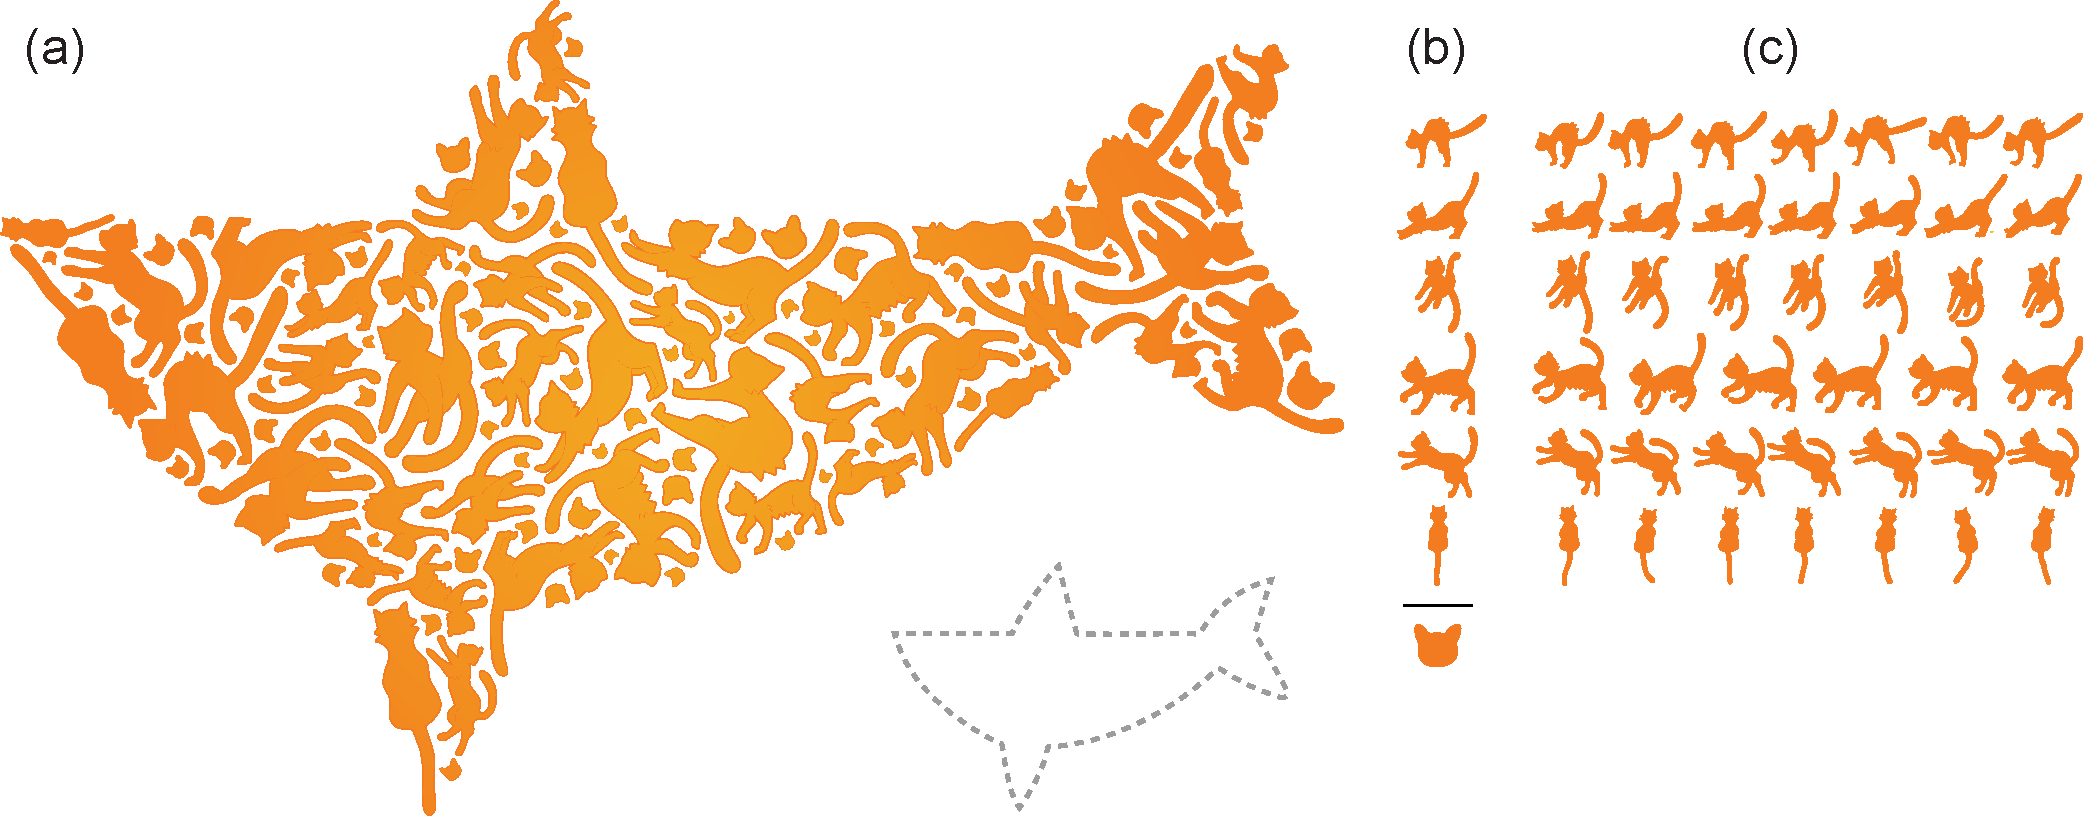
\includegraphics[width=1.0\textwidth]{figures/repulsionpak/cat_whale_04}
  \caption[A packing of a cat]
  {
  \label{cat_packing}
           A packing of six cat elements inside a fish-shaped target container. 
           Controllable deformation and repulsion forces allow the elements to deform,
           efficiently filling the container and creating a uniform distribution of
           negative space. We then reduce the remaining negative space by placing smaller
           cat heads. The gradient fill was added as a post-process.}
\end{figure*}



%%%%%%%%%%%%%%%%%%%%%%%%%%%%%%%%%%%%%%%%%%%%%%%%%%%%%%%%%%
%%%%%%%%%%%%%%%%%%%%%%%%%%%%%%%%%%%%%%%%%%%%%%%%%%%%%%%%%%
\section{Introduction}
\label{repulsionpak_introduction}
%%%%%%%%%%%%%%%%%%%%%%%%%%%%%%%%%%%%%%%%%%%%%%%%%%%%%%%%%%
%%%%%%%%%%%%%%%%%%%%%%%%%%%%%%%%%%%%%%%%%%%%%%%%%%%%%%%%%%



%%%%%%%%%%%%%%%%%%%%%%%%%%%%%%%%%%%%%%%%%%%%%%%%%%%%%%%%%%
%%%%%%%%%%%%%%%%%%%%%%%%%%%%%%%%%%%%%%%%%%%%%%%%%%%%%%%%%%
\section{Previous Work}
\label{repulsionpak_previous_work}
%%%%%%%%%%%%%%%%%%%%%%%%%%%%%%%%%%%%%%%%%%%%%%%%%%%%%%%%%%
%%%%%%%%%%%%%%%%%%%%%%%%%%%%%%%%%%%%%%%%%%%%%%%%%%%%%%%%%%


%%%%%%%%%%%%%%%%%%%%%%%%%%%%%%%%%%%%%%%%%%%%%%%%%%%%%%%%%%
%%%%%%%%%%%%%%%%%%%%%%%%%%%%%%%%%%%%%%%%%%%%%%%%%%%%%%%%%%
\section{System Overview}
\label{repulsionpak_system_overview}
%%%%%%%%%%%%%%%%%%%%%%%%%%%%%%%%%%%%%%%%%%%%%%%%%%%%%%%%%%
%%%%%%%%%%%%%%%%%%%%%%%%%%%%%%%%%%%%%%%%%%%%%%%%%%%%%%%%%%




\begin{figure}[h]
\centering
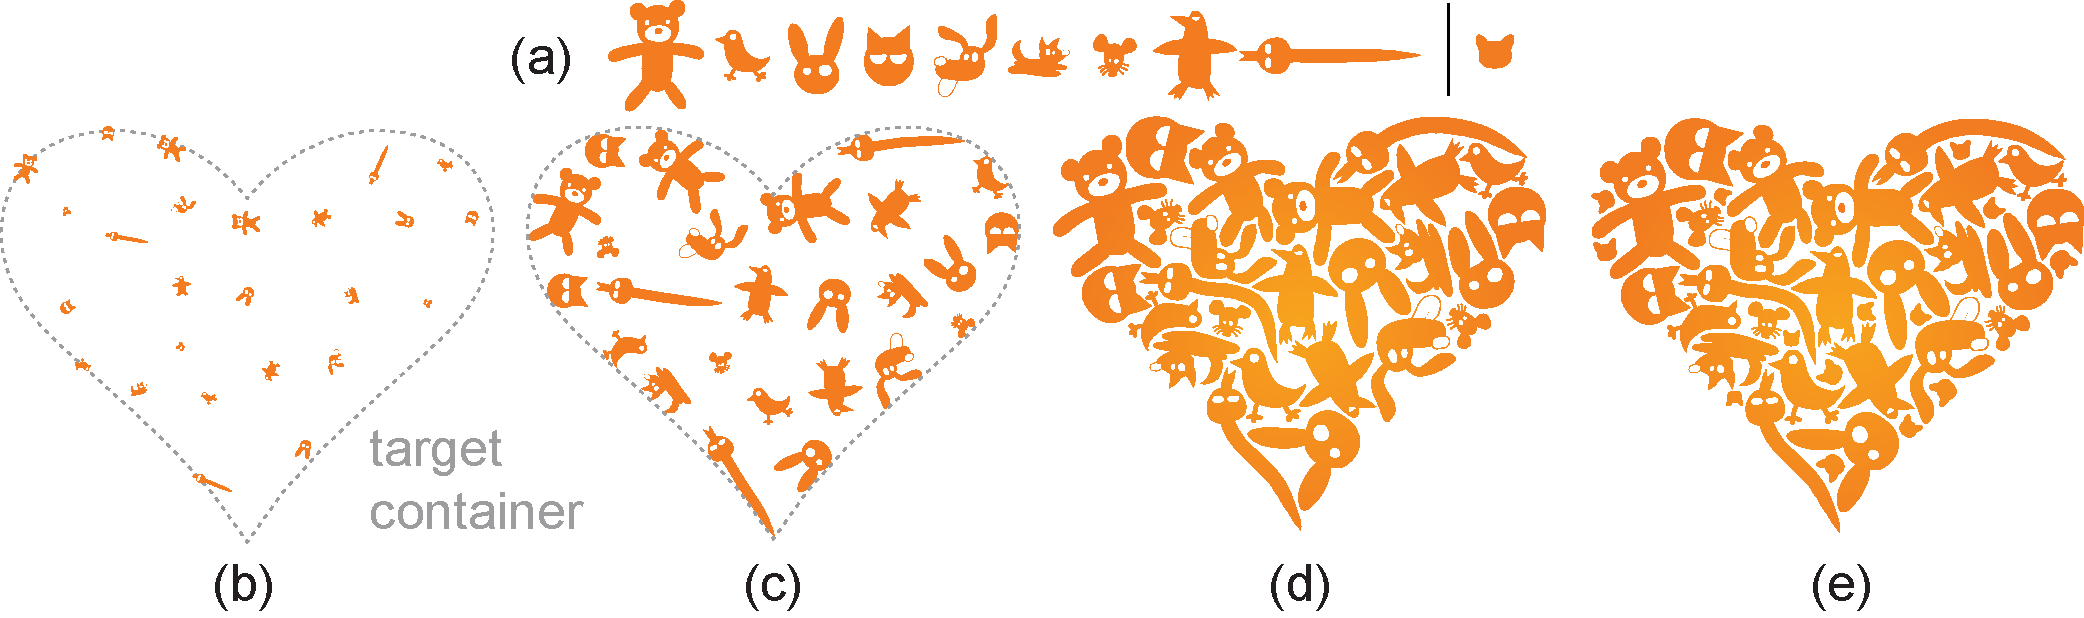
\includegraphics[width=1.0\textwidth]{figures/repulsionpak/pipeline.pdf} 
\caption[RepulsionPak pipeline]
{\label{fig_repulsionpak_pipeline} 
The creation of a packing using RepulsionPak.
  (a) A library of elements, comprising nine primary elements and a single
  	secondary element.
  (b) A target container with the initial distribution of scaled-down elements.
  (c) The simulation in progress, showing the elements growing, translating,
  	rotating, and deforming.
  (d) The resulting packing of primary elements.
  (e) The final result, after adding secondary elements and allowing them to
  	grow.
  	Fig.~\ref{fig_defviz} shows the deformations of some of the elements. }
\end{figure}

\begin{figure}[h]
\centering

\includegraphics[width=5cm]{figures/repulsionpak/pipeline_defviz_csk.pdf}
\caption[Element deformation]{
	\label{fig_defviz}
	Some of the elements in the final packing in Fig.~\ref{fig_repulsionpak_pipeline}, 
	showing the effect of deformation in our simulation.
}
\end{figure}

Our system requires three main pieces of input:
\begin{itemize}
	\item A library of primary and optional secondary elements, such
		as those shown in Fig.~\ref{fig_repulsionpak_pipeline}a.
	      Each element is a collection of 
		  open or closed polygonal paths---any curves must
		  be flattened ahead of time.
	\item One or more closed polygonal target containers, such as the
		heart in Fig.~\ref{fig_repulsionpak_pipeline}b.  Target containers can optionally
		have internal holes.
	\item The desired element spacing distance $d_\mathrm{gap}>0$.
\end{itemize}

RepulsionPak starts by preprocessing the elements, creating additional space around
each to enforce the spacing distance, and fitting a triangle mesh over each element.
\newtext{The containers are then seeded with randomly placed
copies of scaled-down elements 
(Section~\ref{repulsionpak_preprocessing}).}

\newtext{RepulsionPak} then performs a physics simulation on the meshes, 
making them simultaneously grow and repel each other. As a
proof of concept, we implement a spring-based 
simulation, \newtext{which yields satisfactory results despite its simplicity};
many alternatives are possible 
(see Section~\ref{repulsionpak_conclusions}).
Forces in the
simulation push mesh vertices away from vertices in other meshes,
attempt to keep the meshes from undergoing excessive deformation, and resolve
places where meshes overlap or vertices move outside target containers
(Section~\ref{repulsionpak_simulation}).

After each iteration of the simulation, meshes grow into adjacent space
if possible, so that they gradually consume the negative space in the container.
At the same time, mesh self-intersections are resolved
(Sections~\ref{repulsionpak_element_growth} and \ref{section_self_intersection_constraint}).
\mynote{delete self intersection section...}

The simulation concludes 
either when the elements occupy a sufficient proportion of the container area, or 
when some number of simulation steps fail to
significantly reduce the negative space
(Section~\ref{repulsionpak_stopping_criteria}).

Finally, an optional second simulation further reduces and evens out the
negative space.  It begins by placing small secondary elements in large
pockets of negative space.  This simulation is the same as the
first, except that vertices of primary element meshes are not allowed to move
(Section~\ref{repulsionpak_secondary_elements}).

Final SVG output is created by using barycentric coordinates to map each element's
paths from the element's initial mesh into the deformed mesh produced through
simulation.


%%%%%%%%%%%%%%%%%%%%%%%%%%%%%%%%%%%%%%%%%%%%%%%%%%%%%%%%%%
%%%%%%%%%%%%%%%%%%%%%%%%%%%%%%%%%%%%%%%%%%%%%%%%%%%%%%%%%%
\section{Preprocessing}
\label{repulsionpak_preprocessing}
%%%%%%%%%%%%%%%%%%%%%%%%%%%%%%%%%%%%%%%%%%%%%%%%%%%%%%%%%%
%%%%%%%%%%%%%%%%%%%%%%%%%%%%%%%%%%%%%%%%%%%%%%%%%%%%%%%%%%

\begin{figure}[t] %%% ELEMENT IMAGE
\centering
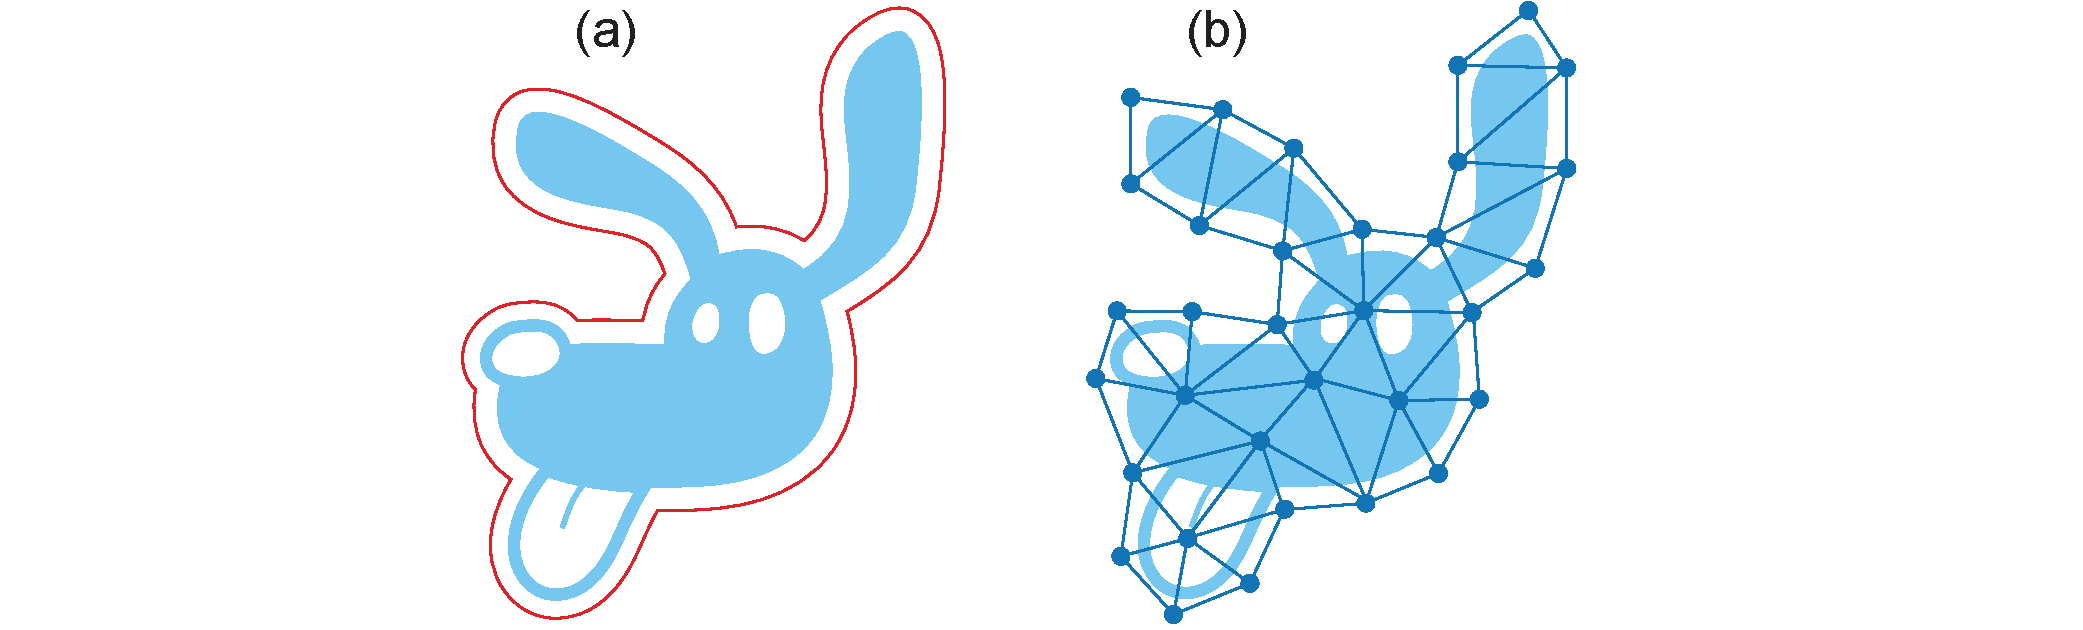
\includegraphics[width=4.5cm]{figures/repulsionpak/element_skin_triangles_2.pdf}
\caption[Element discretization]{
	\label{fig_elements_image}
	\newtext{An illustration of element discretization for preprocessing.}
	(a) An element with its boundary displaced to create a skin, drawn in red.
	(b) A triangle mesh with boundary vertices on the skin.
}
\end{figure}

\begin{figure*}[t]
\centering
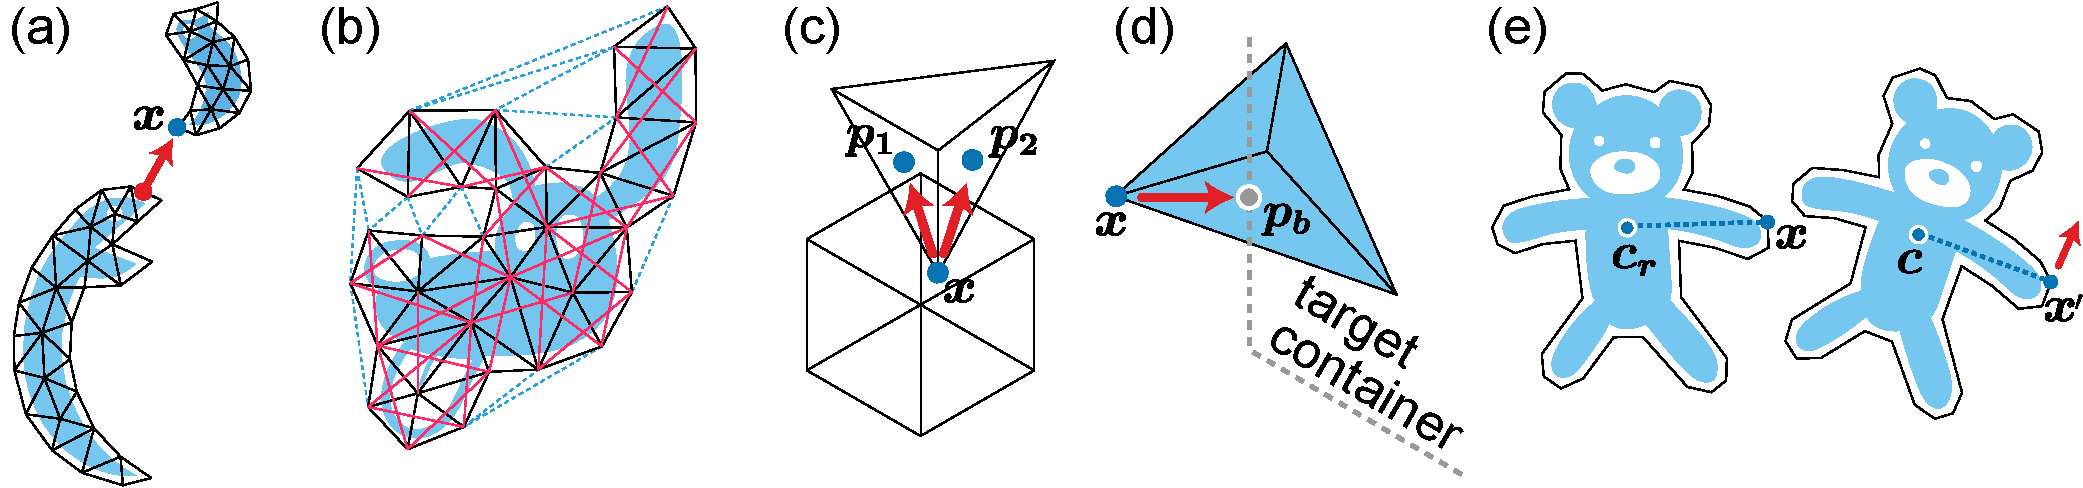
\includegraphics[width=1.0\textwidth]{figures/repulsionpak/all_forces_new.pdf}
\caption[Forces]{
\label{fig_forces}
Illustrations of the forces in our simulation.
\;\textbf{(a)~Repulsion force}:
The closest point on the snake's mesh
repels a vertex $\bm{x}$ in the bird mesh.
\textbf{(b)~Edge force}: 
We generate edge forces using
\newtext{edge springs (black), shear springs (red), and negative-space springs (dashed blue).}
\textbf{(c)~Overlap force}: 
Centres of triangles $\bm{p_1}$ and $\bm{p_2}$ attract a vertex
$\bm{x}$ that lies in the interior of another mesh.
\;\textbf{(d)~Boundary force}: A vertex $\bm{x}$ moves toward $\bm{p_b}$,
the closest point on a target container, when it is outside the container.
\textbf{(e)~Torsional force}: We restrict the orientation of the element by generating 
a torsional force at every boundary vertex $\bm{x}$
to restore its angular position relative to $\bm{c}$, 
the center of mass of the element.
\mynote
{
$\bm{c_r}$
points should be bold.
Should explain negative space edges, and shear edges.
}
}
\end{figure*}


The \textit{skin} of an element is a simple closed polygon 
that fully encloses it, 
as in the red shape in Figure~\ref{fig_elements_image}(a).
We generate the skin 
by offsetting 
an element's boundary outward by $d_\mathrm{gap}/2$. 
The simulation aims to produce an approximate tessellation of the target
container by \newtext{deformed} skins, thereby achieving the desired element spacing and
suppressing overlaps.

We triangulate the element skin to obtain a triangle mesh.
To create the mesh we uniformly sample the skin polygon $s$, with samples
spaced apart by distance $d_\mathrm{gap}$,
to obtain a simpler polygon $s'$ (the outer boundary of the mesh).
We then construct a Delaunay triangulation of $s'$.
The vertices and edges of this mesh become unit 
masses and longitudinal
springs in a physical simulation, allowing elements to deform in response to
their neighbours.  
We further brace the mesh against
deformation by augmenting it with ``auxiliary springs'' (see
Section~\ref{section_forces} and Fig.~\ref{fig_forces}b).

Due to discretization, a low mesh resolution does not guarantee a separation of $d_\mathrm{gap}$. 
Increasing the mesh resolution produces a more precise result at the expense of greater running time.

\textbf{Barycentric coordinates:}
The simulation operates on meshes, not element geometry.  In the final
rendering phase, we will redraw an element relative to a deformed copy of
its mesh.  To do so, we first re-express every vertex of an element path in 
terms of the mesh triangles.  Every element vertex lies either inside a mesh
triangle or just beyond a border edge.  We encode each vertex in barycentric
coordinates relative to its enclosing or nearest triangle.

\textbf{Initial element placement:}
We prepare our simulation by randomly placing non-overlapping elements.
\begin{enumerate}
	\item Generate random points $P = \{ p_1, p_2,..., p_n \}$ 
		  inside the target container 
	      via blue noise sampling~\cite{Bridson2007}.
	      The user controls the number of points; using more points gives results
	      with smaller elements.  We can automatically estimate $n$ by
		  dividing the container area by the desired average area of the element skins.
	\item Cycle through the primary elements, assigning each element to a 
		  random unused $p_i$ with a random orientation, repeating until 
		  every point has an element.
	\item Shrink all the elements so that they do not overlap and occupy only
		  a small fraction of the container's area; in our implementation we
		  have found that $5-10$\% of the area gives good results. Making them
		  larger would speed up the simulation but does
	      not allow enough freedom of movement to generate successful
		  packings.  Fig.~\ref{pipeline}b shows an initial placement.	      
\end{enumerate}


%%%%%%%%%%%%%%%%%%%%%%%%%%%%%%%%%%%%%%%%%%%%%%%%%%%%%%%%%%
%%%%%%%%%%%%%%%%%%%%%%%%%%%%%%%%%%%%%%%%%%%%%%%%%%%%%%%%%%
\section{Simulation}
\label{repulsionpak_simulation}
%%%%%%%%%%%%%%%%%%%%%%%%%%%%%%%%%%%%%%%%%%%%%%%%%%%%%%%%%%
%%%%%%%%%%%%%%%%%%%%%%%%%%%%%%%%%%%%%%%%%%%%%%%%%%%%%%%%%%

We design a simulation in which 
we generate pseudo-physical 
forces that transform elements by transforming their meshes.
Let $\bm{x}$ be a vertex of an element mesh. 
The total force $\bm{F}$ applied to $\bm{x}$ is
\begin{equation}
\bm{F} = \simforce{r} + \simforce{e} + \simforce{b} + \simforce{o} + \simforce{t}
\end{equation}
where $\simforce{r}$, $\simforce{e}$, $\simforce{b}$, $\simforce{o}$ and $\simforce{t}$ are 
the repulsion force, the edge force, the boundary force, the overlap force, \newtext{and the torsional force}.
These forces combine with the growth process, described in
Section~\ref{section_growing_element}, to completely fill the target container.

%%%%%%%%%%%%%%%%%%%%%%%%%%%%%%%%%%%%%%%%%%%%%%%%%%%%%%%%%
%%%%%%%%%%%%%%%%%%%% REPULSION FORCE %%%%%%%%%%%%%%%%%%%%
%%%%%%%%%%%%%%%%%%%%%%%%%%%%%%%%%%%%%%%%%%%%%%%%%%%%%%%%%

%% CSK TODO: what counts as a "nearest neighbouring mesh" in this context?
%% How do we know which neighbours to iterate over?

\medskip
\textbf{Repulsion force:} 
The repulsion force tries to push element meshes apart when they approach
each other, with the goal of
making them transform to align their boundaries (Fig.~\ref{fig_forces}a).
 
The vertex $\bm{x}$ will
experience an inverse square repulsive force, inspired by Coulomb's law,
from all nearby meshes.  We use the following formula:

\begin{equation}
\simforce{r} = k_r \sum_{i = 1}^{n} \frac{\bm{u}}{\| \bm{u} \| }\frac{1}{\varsigma  +\| \bm{u} \|^2 }
\end{equation}
where 
\begin{packeddescriptions}
	\item[$k_r$]        is the strength of the repulsion force relative to
						other forces in the simulation.
	\item[$n$]        is the number of nearest neighbouring meshes to $\bm{x}$. 
	\item[$\bm{x_{i}}$] is the closest point on the skin of the $i$th neighbour.
	\item[$\bm{u}$]  $= \bm{x} - \bm{x_{i}}$
	
						% mesh from $\bm{x}$.		
	
	\item[$\varsigma$]   is a \textit{soft parameter}; it places an upper 
						bound on the magnitude of $\simforce{r}$, avoiding
						explosive instability when $\| \bm{u} \|$ is very small.
\end{packeddescriptions}

An imbalance in the repulsion forces across a mesh's vertices will
naturally induce translation and rotation in meshes, helping their
boundaries discover compatible segments and consuming more of the
remaining negative space.

If $\bm{x}$ lies inside of another element's mesh, then the aggregate repulsion
force from other neighbours can push $\bm{x}$ further inside and
worsen the overlap.  If we discover such an overlap, we set
$\simforce{r}$ to $0$ and use the overlap force $\simforce{o}$, discussed below, to
correct it.

%%%%%%%%%%%%%%%%%%%%%%%%%%%%%%%%%%%%%%%%%%%%%%%%%%%%
%%%%%%%%%%%%%%%%%%%% EDGE FORCE %%%%%%%%%%%%%%%%%%%%
%%%%%%%%%%%%%%%%%%%%%%%%%%%%%%%%%%%%%%%%%%%%%%%%%%%%
\medskip
\textbf{Edge force:} 
%\deadtext{By converting element meshes into mass-spring systems,
%we allow elements to undergo deformation in response to repulsion forces
%exerted by neighbours.  A mesh's edges become longitudinal \textit{edge springs}.}
A mesh's edges are treated as longitudinal \textit{edge springs};
displacement
of these springs allows a mesh to deform in response to repulsion forces
by neighbouring meshes.
In addition, when two mesh triangles share an edge we connect the two vertices
opposite the edge with an \textit{auxiliary spring} (Fig.~\ref{fig_forces}b), 
adding extra bracing to a mesh to prevent it from folding.

An undeformed element mesh provides the rest lengths for all of
its springs; as mesh vertices move relative to each other, the springs
attempt to restore these rest lengths.  Let $\bm{x_{a}}$ and $\bm{x_{b}}$ be
mesh vertices connected by a spring.  We compute the spring force as follows:
% As we apply forces to the masses, springs get shorter or longer, causing
% the element to deform. The edge forces attempt to restore the springs
% back to their rest lengths. 
% If a pair of masses $\bm{x_a}$ and $\bm{x_b}$ are connected by a spring,
% the edge force $\simforce{e}$ is applied to to the mass $\bm{x_a}$, 
% and $-\simforce{e}$ is applied to to the mass $\bm{x_b}$:

\begin{equation}
\simforce{e} =  k_{e} \frac{\bm{u}}{\| \bm{u} \|} s \; ( \| \bm{u} \| - \ell)^2
\end{equation}
where
\begin{packeddescriptions}
	\item[$k_e$] is the strength of the edge force relative to other forces.
	\item[$\bm{u}$] $= \bm{x_{b}} - \bm{x_{a}}$
	\item[$\ell$] is the rest length of the spring.
	\item[$s$] is +1 or -1, according to whether $(\| \bm{u} \| - \ell)$ 
		is positive or negative.
\end{packeddescriptions}

We apply $\simforce{e}$ to $\bm{x_{a}}$ and $-\simforce{e}$ to $\bm{x_{b}}$.
The equation is a modification of Hooke's law
in which the strength of the force increases quadratically
with displacement.
This change allows the meshes to resist severe deformations
when subjected to powerful forces.

% \paul{Also needed: Why two kinds of springs?  Why are edge springs not enough?
% Why do you call it a bending spring?}

%%%%%%%%%%%%%%%%%%%%%%%%%%%%%%%%%%%%%%%%%%%%%%%%%%%%%%%
%%%%%%%%%%%%%%%%%%%% OVERLAP FORCE %%%%%%%%%%%%%%%%%%%%
%%%%%%%%%%%%%%%%%%%%%%%%%%%%%%%%%%%%%%%%%%%%%%%%%%%%%%%

%% CSK TODO: verify that "centroid" is the right word here.

\medskip
\textbf{Overlap force:}
Occasionally, a vertex $\bm{x}$ from one mesh can be pushed inside the skin of a
neighbouring mesh.  In such cases, we temporarily disable the repulsion force
on this vertex
by setting it to 0, and instead apply an overlap force that attempts to
eject the intruding vertex.  In particular, every mesh triangle having $\bm{x}$
as a vertex will pull $\bm{x}$ in the direction of its centroid.  The overlap
force is thus given by:

\begin{equation}
\simforce{o} = k_o \sum_{i = 1}^{n} (\bm{p_{i}} - \bm{x})
\end{equation}
where
\begin{packeddescriptions}
	\item[$k_o$] is the relative strength of the overlap force.
	\item[$n$] is the number of mesh triangles that have $\bm{x}$ as a vertex.
	\item[$\bm{p_{i}}$] is the centroid of the $i$th triangle incident on $\bm{x}$.
\end{packeddescriptions}

The overlap force is zero for vertices that are not within another mesh.

%%%%%%%%%%%%%%%%%%%%%%%%%%%%%%%%%%%%%%%%%%%%%%%%%%%%%%%%
%%%%%%%%%%%%%%%%%%%% BOUNDARY FORCE %%%%%%%%%%%%%%%%%%%%
%%%%%%%%%%%%%%%%%%%%%%%%%%%%%%%%%%%%%%%%%%%%%%%%%%%%%%%%
\medskip
\textbf{Boundary force:}
The boundary force causes element meshes to stay inside the target container
and conform to its boundary. It applies to any vertex $\bm{x}$ that
is outside the container, and moves the vertex towards the closest point
on the container's boundary, by an amount proportional to the distance to
the boundary:
%%% EQ
\begin{equation}
\simforce{b} = k_{b} (\bm{p_b} - \bm{x})
\end{equation}
where
\begin{packeddescriptions}
	\item[$k_b$] is the relative strength of the boundary force.
	\item[$\bm{p_b}$] is the closest point on the target container to $\bm{x}$.
\end{packeddescriptions}

The boundary force is zero for any point inside the container.

\medskip
\textbf{Torsional force:} 
\newtext{
As forces propagate through an element mesh, the aggregate velocity
vectors of the vertices can induce a rotation of the entire element.
However, some elements may have a preferred orientation,
either for aesthetic reasons or because the shape is comprehensible only at certain orientations.
We introduce a torsional force that
penalizes individual vertices for which the orientation, relative to their
element's center of mass, drifts too far from its initial orientation.
}

\newtext{
Consider a vertex $\bm{x}$ belonging
to an element, and let $\bm{c}_r$ be the element's center of mass in
its undeformed state.  We may define the ``rest orientation'' of
$\bm{x}$ as the orientation of the vector $\bm{u}_r = \bm{x}-\bm{c}_r$.
During simulation we compute the current centre of mass $\bm{c}$ of 
the element and let $\bm{u}=\bm{x}-\bm{c}$.  Then the torsional force
is
}
\newtext{
\begin{equation}
  \simforce{t} =\begin{cases}
    k_t\bm{u}^\perp, & \theta > 0\\
    -k_t\bm{u}^\perp, & \theta < 0
  \end{cases}
\end{equation}
where
\begin{packeddescriptions}
	\item[$k_t$]  is the relative strength of the torsional force.
	\item[$\theta$] is the signed angle between $\bm{u}_r$ and $\bm{u}$;
	\item[$\bm{u}^\perp$] is a unit vector rotated $90^\circ$
		counterclockwise relative to $\bm{u}$; and
\end{packeddescriptions}
}
\newtext{
Using the equation above, $\simforce{t}$ is always perpendicular to $\bm{u}$
and the direction of $\simforce{t}$ points to the left or to the right depending on $\theta$.
Unlike the first four force types, the torsional force is optional.}

%%%%%%%%%%%%%%%%%%%%%%%%%%%%%%%%%%%%%%%%%%%%%%%%%%%%%%%
%%%%%%%%%%%%%%%%%%%% THE SIMULATION %%%%%%%%%%%%%%%%%%%
%%%%%%%%%%%%%%%%%%%%%%%%%%%%%%%%%%%%%%%%%%%%%%%%%%%%%%%

\medskip
\textbf{Simulation details:} 
We use explicit Euler integration to simulate the motions of the mesh vertices under the
forces described above.  Every vertex has a position and a velocity vector; in
every iteration, we update velocities using forces, and update positions using
velocities.  These updates are scaled by a time step $\Delta t$, typically
chosen from the range $[0.01,0.1]$.  A smaller time step results in a more
stable simulation at the cost of additional running time.  We cap velocities
at $5\Delta t$ to dissipate extra energy from the system.

%% CSK TODO: verify these measurements.

The repulsion and overlap forces rely on nearest-neighbour queries on the
set of all vertices.  We accelerate these queries by storing vertices in a
uniform spatial subdivision grid that covers the container.  In our
implementation, cell width and height are $6-10$\% of the larger dimension
of the grid.  
%\deadtext{We identify the neighbours of a vertex $\bm{x}$ by considering}
We define the neighbours of a vertex $\bm{x}$ as
all vertices in a $3\times 3$ window of cells centred on the cell
containing $\bm{x}$. 
%\deadtext{Although this is an approximation, since it can miss 
%distant vertices in the composition, the effect is insignificant because of the
%low magnitude of forces involving these vertices.}
This approximation ignores the negligible interactions between
distant vertices.

The constants $k_r$, $k_o$, $k_b$  $k_e$, and $k_t$ control the relative strengths
of the five forces in the simulation.  They must also be chosen relative to
the time step $\Delta t$ and the overall width and height of the container.
We find that our simulation produces satisfactory results when 
$k_r \approx k_o \approx k_b \geq k_e > k_t$.
%\begin{equation}
%k_r \approx k_o \approx k_b \geq k_e
%\end{equation}
For example, if the container's bounding box is approximately $1000\times 1000$,
then we have obtained good results when $k_r=k_o=k_b=80$, $k_e=40$, and $k_t=1$.  We also
set $\varsigma=1$ to avoid explosive repulsion forces.  Increasing $k_e$
relative to the other forces suppresses deformation, yielding a close approximation
of packing with rigid elements.


%%%%%%%%%%%%%%%%%%%%%%%%%%%%%%%%%%%%%%%%%%%%%%%%%%%%%%%%%%
%%%%%%%%%%%%%%%%%%%%%%%%%%%%%%%%%%%%%%%%%%%%%%%%%%%%%%%%%%
\subsection{Element Growth}
\label{repulsionpak_element_growth}
%%%%%%%%%%%%%%%%%%%%%%%%%%%%%%%%%%%%%%%%%%%%%%%%%%%%%%%%%%
%%%%%%%%%%%%%%%%%%%%%%%%%%%%%%%%%%%%%%%%%%%%%%%%%%%%%%%%%%

RepulsionPak starts with small initial elements to avoid intersections,
and gradually enlarges them until they tightly fill the target
container.  Fig.~\ref{pipeline}c-d shows elements growing and gradually
consuming negative space.  Elements have different intrinsic sizes, which are
respected in the initial placement.  Because they all grow at roughly the
same rate, their relative sizes tend to be maintained.

After each iteration of the physics simulation, the element meshes undergo
a growth step.  If an element mesh has no vertices that lie inside of
neighbouring meshes, it is permitted to grow in this iteration.  A mesh with
overlaps may still grow in subsequent iterations, if local changes to the 
packing open up more negative space.
This approach produces \newtext{slight variations} in skin offsets in the output packing
but the effect \newtext{is negligible.}

We implement growth in the context of the physics simulation by scaling
the rest lengths of a mesh's springs, allowing it to expand as the simulation
progresses.  Every mesh $M$ has a counter $n_M$ that records the number of
times it has grown.  When a mesh is permitted
to grow, we add 1 to the counter.  Then, if $L_i$ is the rest length
of the $i$th spring in the original undeformed mesh, we increase its rest
length to $(1+n_Mk_g\Delta t)L_i$.  The constant $k_g$,
usually 0.01 in our system, controls the growth rate.


%%%%%%%%%%%%%%%%%%%%%%%%%%%%%%%%%%%%%%%%%%%%%%%%%%%%%%%%%%
%%%%%%%%%%%%%%%%%%%%%%%%%%%%%%%%%%%%%%%%%%%%%%%%%%%%%%%%%%
\subsection{Stopping Criteria}
\label{repulsionpak_stopping_criteria}
%%%%%%%%%%%%%%%%%%%%%%%%%%%%%%%%%%%%%%%%%%%%%%%%%%%%%%%%%%
%%%%%%%%%%%%%%%%%%%%%%%%%%%%%%%%%%%%%%%%%%%%%%%%%%%%%%%%%%


We choose one of two criteria to stop the simulation. First, the artist specifies 
the desired positive space ratio at which the simulation immediately terminates.
The ratio should not be set too high, and
we find that most packings have positive space ratios between $45\%$ and $65\%$ depending on the element shapes.
For example, concave elements with long extensions are more difficult to pack, 
so a lower positive space ratio is recommended to generate a satisfactory packing.
Second, we stop the simulation when the element meshes are no longer
able to maneuver enough to consume the remaining negative space. 
After each iteration, we compute an \textit{area fraction} $A$, defined to be the fraction of
the container area taken up by element meshes.  We then compute a measurement
of the recent change in area fraction in a sliding window that covers the $w$
most recent iterations of the system; we use $w=100$.  If $A_0,\ldots,A_w$
are the area fractions in the $w+1$ iterations up to the current one, then we
define

\begin{equation}
\mathrm{RMS} = \sqrt{ \frac{1}{w}\sum_{ i = 1 }^{w} { (A_i - A_{i-1}) }^2}
\end{equation}

We stop iterating when $\mathrm{RMS} < \epsilon$, where $\epsilon$ is $0.01$
in our system.

%%%%%%%%%%%%%%%%%%%%%%%%%%%%%%%%%%%%%%%%%%%%%%%%%%%%%%%%%%
%%%%%%%%%%%%%%%%%%%%%%%%%%%%%%%%%%%%%%%%%%%%%%%%%%%%%%%%%%
\section{Secondary Elements}
\label{repulsionpak_secondary_elements}
%%%%%%%%%%%%%%%%%%%%%%%%%%%%%%%%%%%%%%%%%%%%%%%%%%%%%%%%%%
%%%%%%%%%%%%%%%%%%%%%%%%%%%%%%%%%%%%%%%%%%%%%%%%%%%%%%%%%%

The iteration process described above can leave behind isolated pockets of 
empty space, which will be visible in the final composition.  We imitate the
approach taken by human artists by filling these pockets will small, usually
simple secondary elements.  

We seed the container with secondary elements by finding points
that are far from any existing element mesh.  Specifically, we
compute a discrete approximation of the distance transform of the
negative space. We then create an initial candidate list of all
points for which the distance value is above a threshold $d_\mathrm{min}$, sorted
by decreasing distance.  We consider each of these candidates in turn,
adding it to a final list of seed locations provided that no previously
chosen seed is within distance $d_\mathrm{sep}$ of the candidate.
In our implementation, if the distance transform is computed on a 
$1000\times 1000$ grid fit to the container's bounds, then we typically 
set $5 \leq d_\mathrm{min} \leq 10$ and $d_\mathrm{sep}=10$. 

Next, we assign random secondary elements to these chosen seed
points, scaled down as before to avoid overlaps.  We then run the
simulation and growth process again, but freeze the primary elements:
they exert repulsion forces on secondary elements and can induce
overlaps, but primary mesh vertices cannot move.  The secondary
elements gradually grow to consume some of the remaining negative
space until the packing satisfies the same stopping \newtext{criteria}
described above.

Packings with secondary elements are shown throughout the paper; 
see Figs.~\ref{pipeline}e, \ref{cat_packing}, and \ref{three_packings}.


%%%%%%%%%%%%%%%%%%%%%%%%%%%%%%%%%%%%%%%%%%%%%%%%%%%%%%%%%%
%%%%%%%%%%%%%%%%%%%%%%%%%%%%%%%%%%%%%%%%%%%%%%%%%%%%%%%%%%
\section{Shape Matching}
\label{repulsionpak_shape_matching}
%%%%%%%%%%%%%%%%%%%%%%%%%%%%%%%%%%%%%%%%%%%%%%%%%%%%%%%%%%
%%%%%%%%%%%%%%%%%%%%%%%%%%%%%%%%%%%%%%%%%%%%%%%%%%%%%%%%%%



\begin{figure}[t]
\centering

\includegraphics[width=0.3\columnwidth]{figures/repulsionpak/descriptor_2.pdf}
\caption[A local shape descriptor for shape matching]
{\label{fig_shape_matching}
\newtext{An illustration of a local shape descriptor with $n = 3$. 
These segments have varying arclengths but they all have the same value
of $\tau$, the integral of absolute curvature along their lengths.}
}
\end{figure}
\begin{figure}
\centering
\includegraphics[width=0.95\columnwidth]{figures/repulsionpak/rhino_shape_matching_bitmap.pdf} 
\caption[A demonstration of shape matching of leaf shapes inside a rhinoceros]
{\label{rhino_packing}
{ 
A demonstration of shape matching of leaf shapes inside a rhinoceros. 
(a) We detect nine salient features, namely sharp convex corners, and 
assign an element to each.
(b) A spring holds each element in place.
(c) The final result.
}
}
\end{figure}

The motions and deformations of elements, as described
in the previous sections, give them an opportunity to conform to each 
other and to the target container.  However, in some cases the random 
seeding may position some elements in such a way that the simulation 
process will still leave undesirable artifacts.  In particular, when
a round element is placed near a sharp convex corner of the container,
it cannot deform enough to extend into the corner, but cannot yield its
position to a pointy element that offers a better fit.  In the final
packing, the sharp corners of the containers will appear ``rounded off''.
Another problem occurs when a long narrow element is initially placed diagonally across a corner, 
in which case the simulation pushes the element's middle into the corner, causing extreme deformation.

To overcome these deficiencies, we optionally perform an initial fit-guided
placement pass before seeding the rest of the container at random. 
Here we take inspiration from existing rigid packing 
algorithms~\cite{Kwan2016}, which are driven primarily by shape 
compatibility.  We use a simplified shape descriptor; we can tolerate
a less perfect initial fit, with the expectation that deformation will
improve the quality later.

We begin by building shape descriptors for the elements.  
Each element is first scaled to have area
$0.6A_c/n_e$, where $A_c$ is the container area and $n_e$ is the 
number of elements.  This step resizes the element to a rough estimate
of its final size in the packing, an approximation that is adequate
for our fit-based placement.  We then sample the target container and
the boundaries of the elements, with adjacent samples separated by
distance $\delta$.  We set $\delta=0.002L_s$, where $L_s$ is the
side length of the container's bounding square.

We define a local descriptor based on integral of absolute curvature~\cite{Cui2009,Kwan2016}.
Let $P(t)$ be an arclength-parameterized 2D curve, and let $\kappa(t)$ represent the curvature of the curve at $P(t)$.  For a given interval $[s,t]$ within the curve's domain, we may define the integral of absolute curvature
$\tau(s,t) = \int_{s}^{t} | \kappa(x) | dx$.

In practice, we estimate curvature from the discrete sample points
using second-order forward finite differences~\cite{Banchoff} 
and compute $\tau$ by summing curvature estimates using the trapezoid rule.

Let an objective $\tau_\mathrm{obj}$ be a positive real number and $P(t_0)$ be a given point on a curve.  If $\tau_\mathrm{obj}$ is sufficiently small, then as we traverse the curve on either side of $P(t_0)$ we will eventually reach points $P(t_{-1})$ and $P(t_1)$ such that $\tau(t_{-1},t_0)=\tau(t_0,t_1)=\tau_\mathrm{obj}$.  We let $l_1=t_0-t_{-1}$ and $r_1=t_1-t_0$ be the arclengths that produce these integrals.  We can continue this process for any number of steps, walking in both directions along the curve away from previous sample points until we reach $\tau_\mathrm{obj}$, yielding new arclengths $l_k$ and $r_k$ (see Fig.~\ref{fig_shape_matching}).  Finally, for a given number of steps $n$ we define the shape descriptor at $P(t_0)$ as
$(l_n, l_{n-1}, \ldots, l_2, l_1, r_1, r_2, \ldots, r_{n-1}, r_n)$.
Like PAD~\cite{Kwan2016}, our shape descriptor is rotation 
invariant.  Effectively it is one level of a PAD, which suffices because
we do not require scale invariance.
Descriptors can be compared using simple Euclidean distance, accelerated
by storing them in a k-D tree.
In our implementation we set $\tau_\mathrm{obj}=0.001L_s$; the dependence
on $L_s$ makes the measurement robust against changes in absolute container
size, and the factor of $0.001$ was determined through experimentation.
We further choose $n=5$, yielding a 10-dimensional descriptor. We compute
this descriptor for all the container and element samples defined above.

Based on these descriptors, we now use a simple greedy heuristic to identify salient container features where shape matching will be used.
Here we restrict our attention to convex protrusions with high curvature, which benefit the most from careful element placement (See Fig.~\ref{rhino_packing}a).  Given a shape descriptor, we define its total length to be $\sum_{i=1}^nl_i+r_i$.  We iterate over all sample points on the container boundary in increasing order by the total lengths of their descriptors.  For each sample point $P(t_0)$, we add it to a list of salient features under two conditions. First, we require that the angle formed by $P(t_0)$ with two samples to either side of it be sufficiently acute; we use a threshold of 0.3 radians to ensure convex-to-convex matching.
Second, we ensure that salient features are not too close to each other by requiring that every new sample point be separated by a distance of at least $0.2L_s$ from all previously identified salient features.

Even when an element's descriptor is a close match to a segment of 
target container, 
it may still not be safe to place that element at a given location.
For example, one part of an element may extend into a corner of the container,
while a different part, outside the purview of the local shape descriptor,
could protrude outside the container entirely.  We augment our 
descriptor-based fit calculation with an additional score adapted from
Gal et al.~\cite{Gal2007B} in order to ensure a more global element fit.
Let $d(\bm{x})$ be a signed distance function for the container, with
negative values inside the container and positive outside.  In practice we
superimpose a $1000\times 1000$ grid over the container's bounding square and
compute a discrete approximation of the distance transform.  For an element
sample point $\bm{x}$, we then compute a score
\begin{equation}
 q(\bm{x}) =\begin{cases}    
    e^{-\nicefrac{d(\bm{x})^2}{\mu^2\beta}}, & \mathrm{if} \;\; d(\bm{x}) < 0 \\
    1, & \mathrm{if} \;\;d(\bm{x}) = 0 \\
    - \alpha d(\bm{x}), & \mathrm{if}\;\; d(\bm{x}) > 0    
  \end{cases}
\end{equation}

With this scoring function, a sample point that lies on the container boundary
will have a score of 1, the maximum for $q(\bm{x})$.
Scores decay exponentially towards 0
for points farther inside the container.  Sample points outside the container
are penalized by assigning a negative score proportional to distance.

We then define a quality measurement for an entire element by summing over
all of its sample points:
\begin{equation}
Q = \sum_{i = 1}^{n_p} q(\bm{x}_i)
\end{equation}
The parameter $\alpha$ penalizes elements with parts that protrude outside
the container; $\beta$ favors elements with parts close to the target container; 
$\mu = 0.5 \sqrt{2}L_{s}$ is half of the diagonal of the container's
bounding square; and $n_p$ is the number of sample points on the element.
In our implementation we choose $\alpha = 1$ and $\beta = 0.001$.
For every salient container feature, we obtain the $10$ closest descriptors from the k-D tree, and choose one that has the highest $Q$.
Finally, we place the selected element in the container by 
aligning the endpoints of the element's and container's matching shape 
descriptors.

The shape matching process yields a set of elements that should be attached
to particular locations on the target container.  However, during simulation
they could wander away from these initial positions, under the influence of
the many other forces at play.  As shown in Fig.~\ref{rhino_packing}b, we
encourage these elements to remain in place by attaching them to the salient
container points with additional springs.

%%%%%%%%%%%%%%%%%%%%%%%%%%%%%%%%%%%%%%%%%%%%%%%%%%%%%%%%%%
%%%%%%%%%%%%%%%%%%%%%%%%%%%%%%%%%%%%%%%%%%%%%%%%%%%%%%%%%%
\section{Results}
\label{repulsionpak_results}
%%%%%%%%%%%%%%%%%%%%%%%%%%%%%%%%%%%%%%%%%%%%%%%%%%%%%%%%%%
%%%%%%%%%%%%%%%%%%%%%%%%%%%%%%%%%%%%%%%%%%%%%%%%%%%%%%%%%%



\begin{figure*}
\centering
\includegraphics[width=1.0\textwidth]{figures/repulsionpak/allresults.pdf} 
\caption[Three packings created using RepulsionPak: Birds, Bats, and Butterflies]
{\label{three_packings} Three packings created using RepulsionPak: \newline Birds, Bats, and Butterflies. The results are visually appealing overall,
though some birds' tails suffer from excessive deformation in
the packing on the left.}
\end{figure*}

\begin{figure*}
\centering
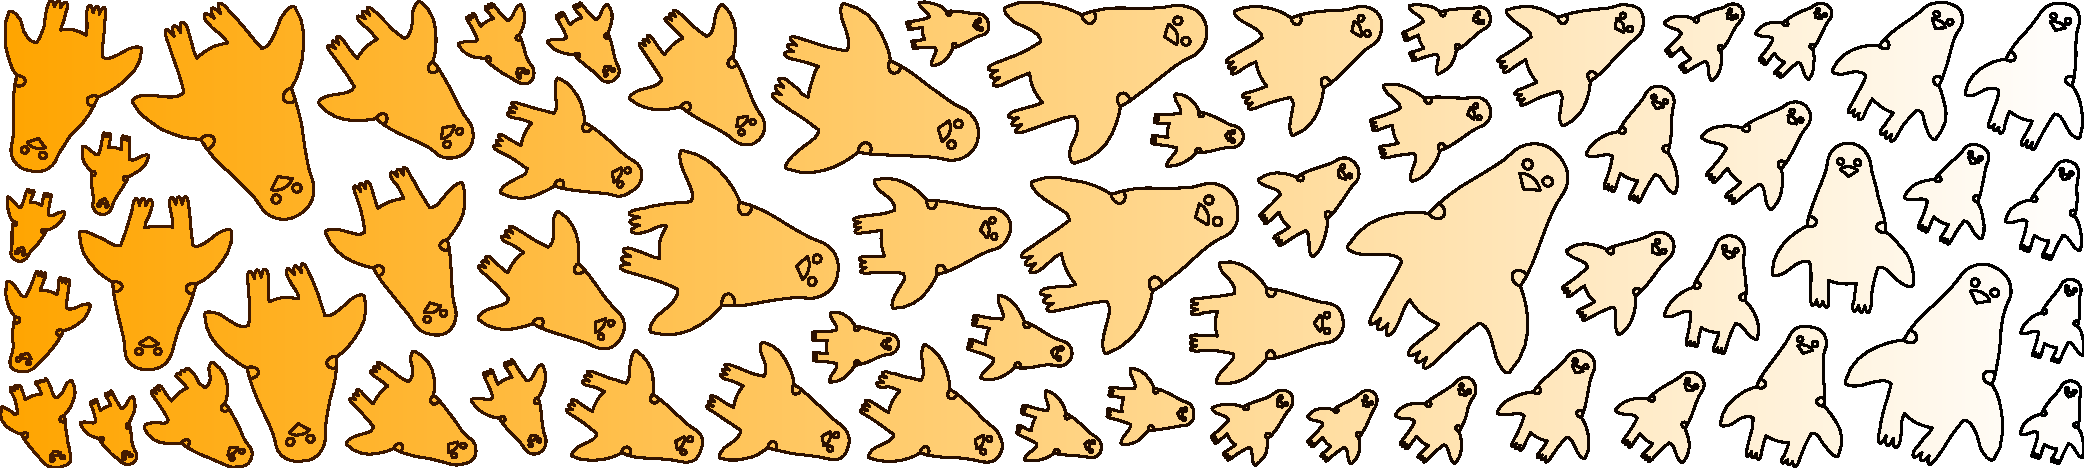
\includegraphics[width=1.0\textwidth]{figures/repulsionpak/giraffe_penguin.pdf}
\caption[A packing that demonstrates torsional forces]
{\label{giraffe_penguin_packing}
A packing that demonstrates torsional forces.
The packing uses copies of a single element shape, but every copy is given a rest orientation between $0^\circ$
and $180^\circ$, based on its horizontal position in the container.  In the final packing the elements transition
from upright to upside-down, recreating an illusion in which giraffe heads become penguins.}
\end{figure*}

%\begin{minipage}{\textwidth}
\begin{figure}
\centering
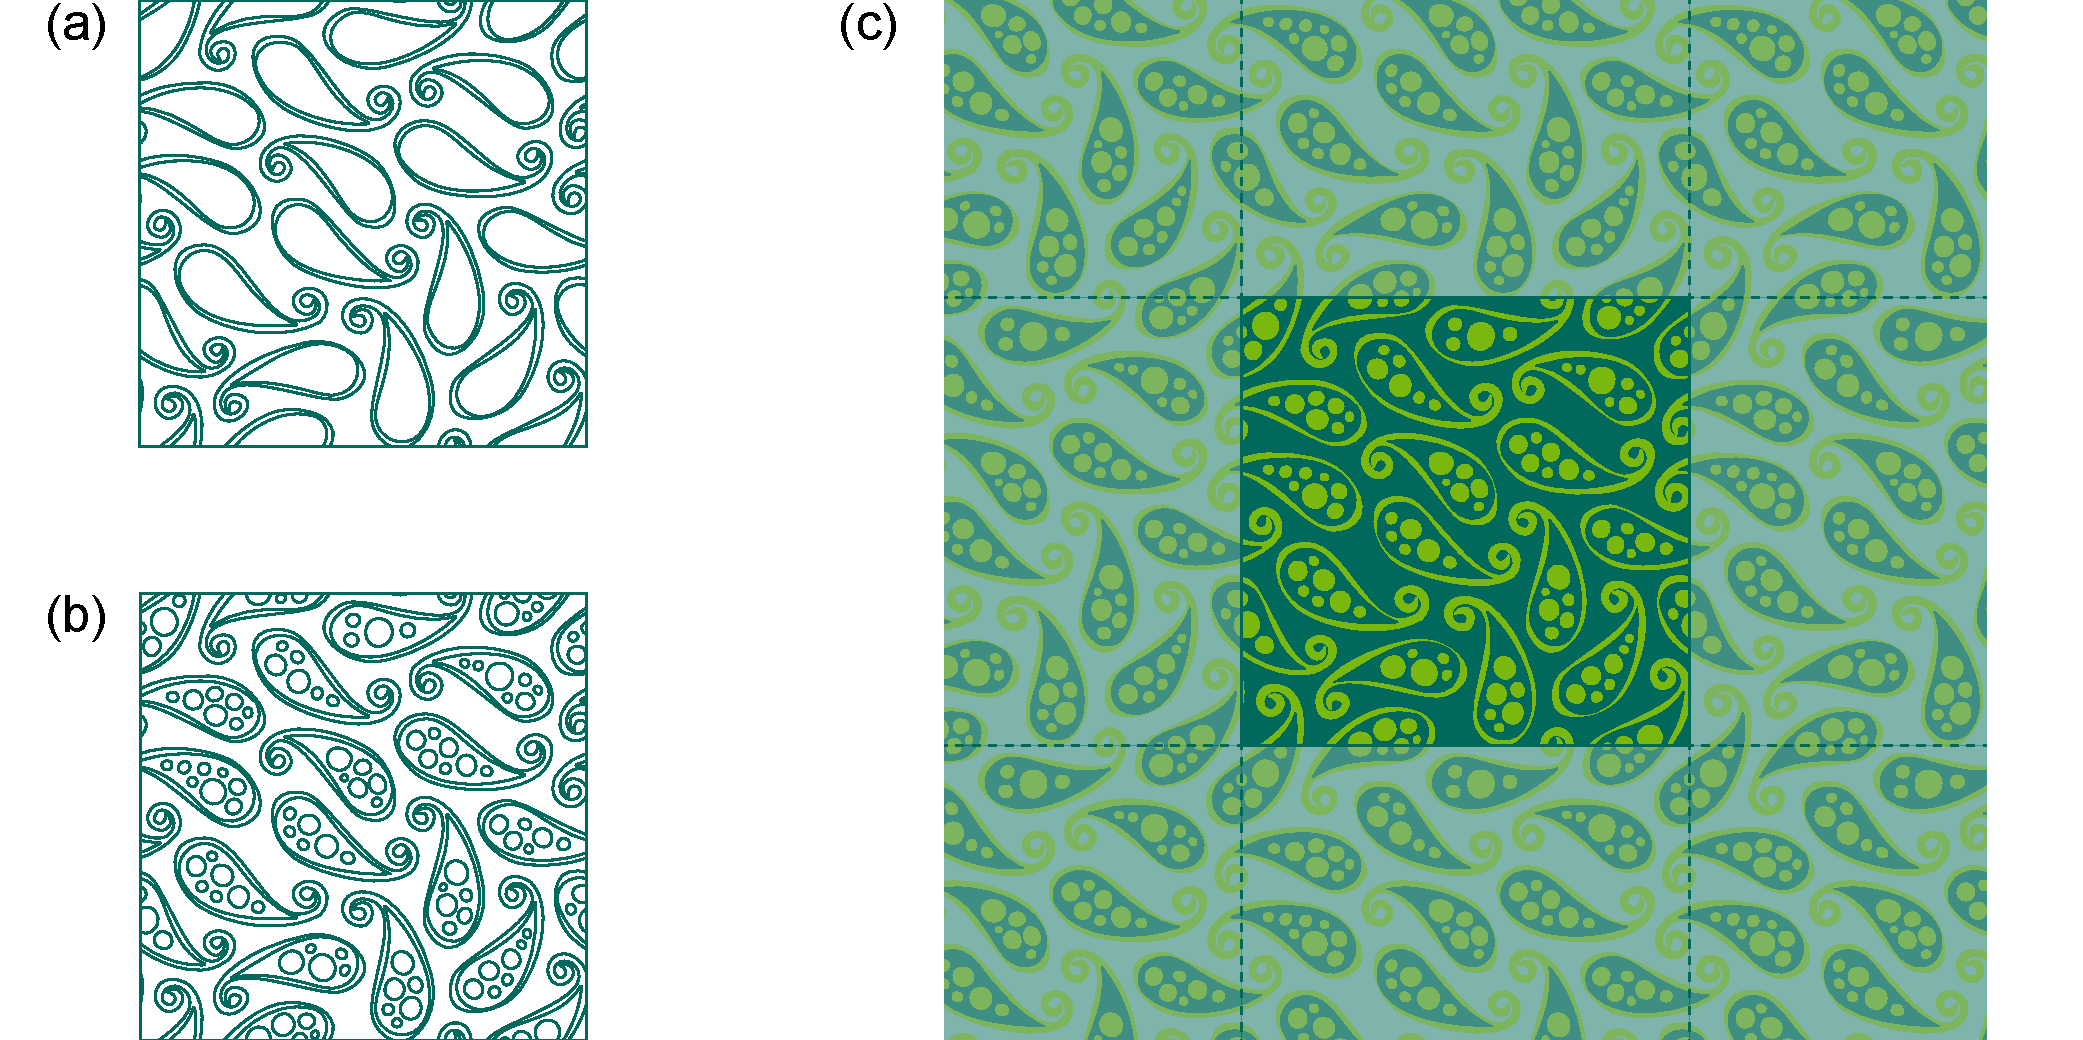
\includegraphics[width=0.95\columnwidth]{figures/repulsionpak/paisley_new.pdf} 
\vspace{-10pt}
\caption[A paisley-inspired toroidal packing that can tile the plane]
{\label{paisley_packing}
A paisley-inspired toroidal packing that can tile the plane. 
           (a) An initial paisley packing.
           (b) In a separate simulation, we fill each paisley with circles to demonstrate a packing inside a packing.
           (c) The final result.
}
\end{figure}

\begin{figure}
\centering

\includegraphics[width=0.85\columnwidth]{figures/repulsionpak/bad_results.pdf} 
\vspace{-12pt}
\caption[Two demonstrations of how extreme parameter values can lead to \newline 
	low-quality results]
	{\label{bad_results}
Two demonstrations of how extreme parameter values can lead to
	low-quality results.  In~(a), we allow repulsion to overwhelm element
	shape by setting $k_r$ to 200 and $k_e$ to 20; the resulting packing 
	has even negative space, but elements suffer from high deformation
	and self intersections.  In~(b), we minimize repulsion and prioritize
	orientation by setting $k_e$, $k_t$, and $k_r$ to 200, 100, and 50,
	respectively.  The elements deviate minimally from their original shapes 
	and orientations, but cannot fill the container effectively.
}
\end{figure}

\begin{table}[h]
\centering 
\caption[Data and statistics for the RepulsionPak results]
{
   Data and statistics for the RepulsionPak results.  The table shows the
   numbers of primary and secondary elements ($n_p$, $n_s$),
   the number of vertices ($v$), 
   the running times of the primary and the secondary simulations ($t_p$, $t_s$) in seconds,
   and the number of iterations ($i$).
   In these results, torsional forces are used only in 
   Fig.~\ref{giraffe_penguin_packing} and shape matching is used only 
   in Fig.~\ref{rhino_packing}.
   }
\label{packing_statistics}
\definecolor{lg}{rgb}{0.73,0.867,0.98}
\vspace{-10pt}
\resizebox{\columnwidth}{!}{
\begin{tabular}{|l|c|c|c|c|c|c|}
\hline
\cellcolor{lg}Packing                  & \cellcolor{lg}$n_p$ & \cellcolor{lg}$n_s$ & \cellcolor{lg}$v$   & \cellcolor{lg}$t_p$ & \cellcolor{lg}$t_s$ & \cellcolor{lg}$i$\\ \hline
Animals (Fig.~\ref{pipeline})                       & 25    & 14   & 2412  & 133  & 65  & 16670\\ \hline
\newtext{Rhino   (Fig.~\ref{rhino_packing})}        & 107   & 0    & 4833  & 237  & 0   & 15521\\ \hline
Cats (Fig.~\ref{cat_packing})                       & 41    & 69   & 3598  & 185  & 62  & 8531\\ \hline
Birds  (Fig.~\ref{three_packings}a)                 & 43    & 43   & 2309  & 102  & 54  & 11571\\ \hline
Bats (Fig.~\ref{three_packings}b)                   & 47    & 22   & 3048  & 165  & 56  & 13120\\ \hline
Butterflies (Fig.~\ref{three_packings}c)            & 123   & 135  & 11916 & 696  & 616 & 14379\\ \hline
\newtext{Giraffes \& Penguins (Fig.~\ref{giraffe_penguin_packing})}        & 60    & 0   & 2250  & 163  & 0   & 9347\\ \hline
\newtext{Paisley (Fig.~\ref{paisley_packing})}      & 162   & 0    & 4860  & 128  & 0   & 23040\\ \hline
\newtext{Circles in Paisleys (Fig.~\ref{paisley_packing})}      & 144   & 0    & 2544  & 403  & 0   & 29584\\ \hline
\newtext{Collage (Fig.~\ref{pad_comparison})}       & 51    & 0    & 3481  & 729  & 0   & 29868\\ \hline
\newtext{Autumn  (Fig.~\ref{balabolka_comparison})} & 77    & 0    & 2427  & 868  & 0   & 38387\\ \hline
\end{tabular}
} 
\end{table}


Our software was written in C++, and reads in text files describing
elements and containers; we prepared these files using
Adobe Illustrator.  We ran
our software on a computer with a 2.4 GHz Intel i7-4700HQ processor
and 16 GB of RAM.  As a post-process, we optionally read packings
back into Illustrator, fit smooth curves to polygonal paths, and
apply colours and other visual effects.  Table~\ref{packing_statistics}
shows statistics for the results in the paper.  All results in this
paper use $\Delta t = 0.1$.
Torsional forces are used only in Fig.~\ref{giraffe_penguin_packing},
and shape matching is used only in Fig.~\ref{rhino_packing}.
We also use our improved method for resolving self intersection in
Figs.~\ref{rhino_packing},~\ref{giraffe_penguin_packing},
~\ref{paisley_packing},
~\ref{pad_comparison}, and
~\ref{balabolka_comparison}.

The supplemental materials include movies that visualize the simulation
process.  These movies make it clear that elements can jostle each other
around, inducing translation, rotation, and deformation throughout the 
simulation.

The packing in Fig.~\ref{cat_packing} 
uses six cat-shaped primary elements and one secondary cat head.
RepulsionPak naturally bends legs and tails to fill the container more evenly.

The animal packing in Fig.~\ref{pipeline} 
has several elements with limbs (the bear, fox, chick, and penguin),  
extensions (the dog and bunny ears), and long shapes (the snake).
Fig.~\ref{fig_defviz} highlights the deformations for some of these elements;
they are noticeably more deformed 
than nearly convex elements like the cat and mouse.


The butterfly packing in Fig.~\ref{three_packings} is an attempt to reproduce 
the visual style of a 
dense packing (or tessellation), similar to Jigsaw Image Mosaics~\cite{Kim2002}
or the ``Butterflies in Butterfly'' example from the
Pyramid of Arclength Descriptor paper~\cite[Fig. 21]{Kwan2016}. 
The target container is made from two regions,
one with internal holes.  The resulting packing is tight but overlap-free.

The packing on the left in Fig.~\ref{three_packings}
exhibits significant deformation in the wings and the tails of the birds.
In particular, the thin tails of the swallows have some unaesthetic
sharp bends.  We would like to investigate ways to ensure these bends are
smoother.

The packing in Fig.~\ref{giraffe_penguin_packing} demonstrates torsional forces
that gradually turn the elements upside down. 
The rhinoceros packing in Fig.~\ref{rhino_packing} demonstrates initial placement via shape matching.
The entire shape matching process took 922 milliseconds with a 4-element library.

We have also experimented with creating tileable packings, as shown
in Fig.~\ref{paisley_packing}.  We seed a central square with elements,
but also place clones of those elements in all the squares of the
8-neighbourhood around the center.  These clones track the transformations
and deformations of their originals, but also exert forces on them during
simulation, leading to an even, seamless packing in a toroidal domain.

We have found that RepulsionPak is robust to parameter variation, and 
produces predictable, high quality results without the need for fine-grained
adjustments.  However, as shown in Fig.~\ref{bad_results}, extreme parameter 
settings can still produce degenerate results.
In Fig.~\ref{bad_results}a, the repulsion force is made much stronger than 
the edge force, leading to excessive element deformation and
self-intersections in the pursuit of even negative space.  In 
Fig.~\ref{bad_results}b, edge and torsional forces dominate repulsion,
producing a packing with stiff, upright elements that do not fill their
container effectively.


%%%%%%%%%%%%%%%%%%%%%%%%%%%%%%%%%%%%%%%%%%%%%%%%%%%%%%%%%%
%%%%%%%%%%%%%%%%%%%%%%%%%%%%%%%%%%%%%%%%%%%%%%%%%%%%%%%%%%
\section{Conclusions}
\label{repulsionpak_conclusions}
%%%%%%%%%%%%%%%%%%%%%%%%%%%%%%%%%%%%%%%%%%%%%%%%%%%%%%%%%%
%%%%%%%%%%%%%%%%%%%%%%%%%%%%%%%%%%%%%%%%%%%%%%%%%%%%%%%%%%

\mynote{need to move a few sentences to evaluation}

We presented RepulsionPak, a method to create packings with deformable elements.
The combination of repulsion forces and controlled deformation
allows RepulsionPak to discover shape compatibilities that
eliminate the need for a large element library
and fill the target container effectively.
\newtext{
Our compositions have negative space between elements that
is approximately uniform in width, and we validate our approach using overlap functions,
spherical contact probability functions, and distance histograms.
}

We see many possibilities for further improvements to RepulsionPak
and future research on element packings.


\begin{itemize}
\item 
	Because our main goal was to demonstrate the validity of a 
	deformation-driven approach, and not to contribute a new
	physical simulation method, we deliberately chose a simple 
	simulation model based on springs and forward Euler integration.
	Contemporary research has yielded many more sophisticated 
	physical simulation methods, such as Position Based Dynamics~\cite{Muller2007}, 
	Projective Dynamics~\cite{Bouaziz2014}, and the Finite Element Method.
	No one method is obviously best suited to this problem, and
	we intend to experiment with several to investigate if any offers
	a suitable trade-off between performance and quality.

\item We would like to explore the use of RepulsionPak in a fabrication context.
      For example, our boundary compatibilities might be used to create a connected object.
      Alternatively, it would be interesting to 3D print the 
      negative space, which is already connected,
	  leaving holes that surround the element shapes.

\item Our barycentric warping method can
	introduce undesirable artifacts in highly deformed elements, as
	in the swallow tails in the left result of Fig.~\ref{three_packings}.
	We would like to explore other methods for warping an element's
	geometry based on the correspondences between the triangles of its original
	mesh and the deformed meshes in the final packing, based for example on the
	work of Jacobson et al.~\cite{Jacobson2011} and Liu et al.~\cite{Liu2014}.

\end{itemize}